
The main fold-out visualization we present (Fig.~\ref{fig:foldout}) is a composition of smaller elements, each a birth distribution. We therefore build up to its full description by making explicit some basic notions of birth distributions and the calendar time line, drawing a distinction between two kinds of birth distributions featured in the final plot. This is intended to aid in the interpretation of the main figure. 

In the period perspective, a picture of the births is for demographers most instinctively broken down by the age of mothers who gave birth in that year, Fig.~\ref{fig:agemother}, or by the year of birth of mothers, Fig.~\ref{fig:cohmother}. These two distributions are essentially identical, but appear as mirror images if chronological time is enforced in $x$. This is key: In the period perspective with births arranged on an age axis, young mothers are on the left and older mothers on the right, but the reverse is true on a cohort axis. Count distributions such as this may be jagged, even if the underlying rate distributions are smooth, due to population structure.\footnote{The deficit around age 31 in \ref{fig:agemother} is due to a smaller number of potential mothers: Cohorts born between 1867 and 1869 were smaller than the surrounding cohorts due to a famine in those years.} 

\begin{figure}[ht!]
\begin{subfigure}[t]{0.5\textwidth}
        \centering
        \includegraphics[width=\textwidth]{Figures/Fig11900MotherAge.pdf}
        \caption{Births in 1900 by age of mother}
        \label{fig:agemother}
\end{subfigure}
~
\begin{subfigure}[t]{0.5\textwidth}
        \centering
        \includegraphics[width=\textwidth]{Figures/Fig11900MotherCohort.pdf}
        \caption{Births in 1900 by year of birth of mother}
          \label{fig:cohmother}
\end{subfigure}
\caption{Births in a year structured by mothers' age versus mothers' year of birth are a
reflection over $y$ and shift over $x$. }
\end{figure}

Given a long-enough time series of births classified by age and/or mother cohort, the full reproductive career of the cohort of individuals born in a particular year can be represented as a distribution (assuming no effects of migration). Since the childbearing of a cohort is spread over a synchronous span of ages and years, the $x$-indexing by age (Fig.~\ref{fig:age1900mother}) or year (Fig.~\ref{fig:year1900}) yields identical and redundant distributions: there is no reflection of young and old mothers when toggling between age and period classifications in the cohort perspective: In both cases young mothers are on the left and older mothers on the right. The distribution of births over the lifecourse of a cohort often resembles the smoothness of fertility rate schedules, but this is not necessarily the case.

\begin{figure}[ht!]
\begin{subfigure}[t]{0.5\textwidth}
        \centering
        \includegraphics[width=\textwidth]{Figures/Fig11900IDAge.pdf}
        \caption{Births from mothers born in 1900 by age of mother}
        \label{fig:age1900mother}
\end{subfigure}
~
\begin{subfigure}[t]{0.5\textwidth}
        \centering
        \includegraphics[width=\textwidth]{Figures/Fig11900IDYear.pdf}
        \caption{Births from mothers born in 1900 by year}
          \label{fig:year1900}
\end{subfigure}
\caption{Births of a cohort structured by mothers' age versus mothers' year of birth are a shift over $x$. }
\end{figure}

The births in a year are classified by mothers' cohort, i.e. cohort \emph{origins} in Fig.~\ref{fig:cohmother}, whereas the births \emph{from} a cohort are classified \emph{to} period in Fig.~\ref{fig:year1900}. The two distributions are different in kind, but relatable and both on a common scale. Importantly, these two distributions are indexed to the same calendar line. A fuller representation of their relationship would place them as two disjoint distributions on the same timeline, as in Fig~\ref{fig:juxt}.

\begin{figure}[ht!]
 \centering
        \includegraphics[width=\textwidth]{Figures/Fig31900juxt.pdf}
        \caption{The cohort distribution of mothers who gave birth in 1900 (\textbf{A}) and the births from mothers born in 1900 by year (\textbf{B}). These two distributions imply \emph{three} generations: the mothers of the 1900 cohort, the cohort of 1900 itself, and the offspring of the 1900 cohort.}
          \label{fig:juxt}
\end{figure}

The two distributions on the calendar axis in Fig.~\ref{fig:juxt} are related, and of comparable scale, but different in kind. The $x$ coordinate of the left distribution \textbf{A} is indexed to mothers' birth cohort (old to young), whereas the $x$ coordinate of the right distribution \textbf{B} is indexed to child cohort, occurrence year (young to old). In this way the respective $x$ coordinates are two generations apart, relating to each other as grandmothers and grandchildren. These are two distributions that we may wish to compare in various ways to better understand the birth series, but doing so for the entire Swedish dataset presents a practical challenge for a single visualization. 

For the case of our extended Swedish birth series, we have 281 distribution pairs such as the year 1900 dual shown in Fig.~\ref{fig:juxt}, making simultaneous rendering impractical unless we transform the data in some way. An honest attempt might look like Fig.~\ref{fig:reflect1}, where we reflect the left distribution \textbf{A} over $y$, keeping \textbf{B} on the top axis. These two distributions are linked by the year 1900, the reference year, which of course overlaps with neither of them. In this representation, distributions \textbf{A} and \textbf{B} are re-drawn for each possible reference year from 1736 to 2016, and therefore imply a large sequential set of overlapping distributions. Each \nth{20} distribution is highlighted, but despite attempts to make this graph legible, i) the high degree of overlapping and ii) the spatial dissociation of each \textbf{A} --- \textbf{B} pair makes the intended comparison difficult over the series. These two drawbacks hide some macro patterns present in the data.

\begin{figure}[ht!]
 \centering
        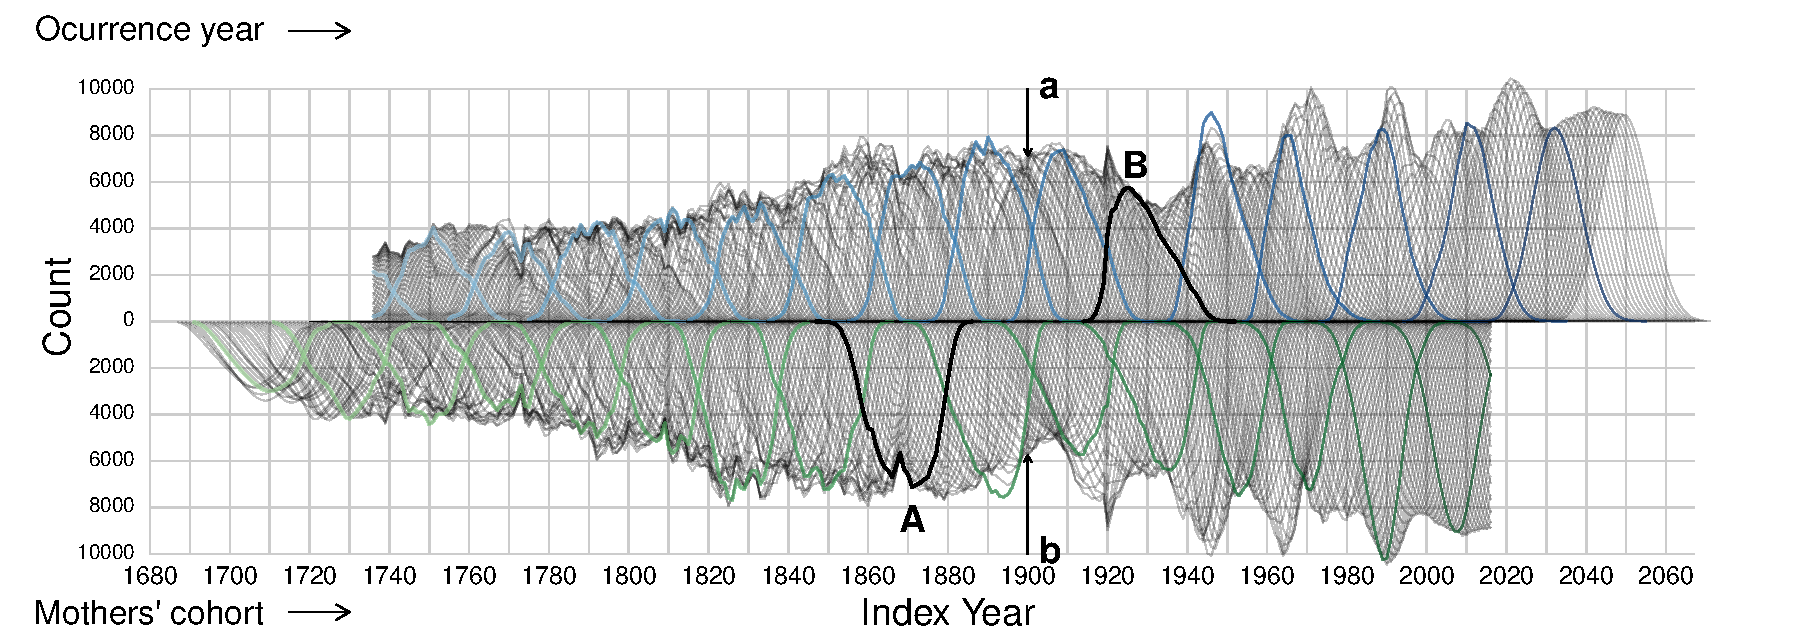
\includegraphics[width=\textwidth]{Figures/FxFlowReflect.pdf}
        \caption{One time series of birth count distributions, under the period and cohort perspectives. The top series is composed of cohort offspring distributions indexed to period. The bottom series is composed of period birth distributions indexed to mothers' cohort. \textbf{A} and \textbf{B} are the same as in Fig.~\ref{fig:juxt}. The cross-section \textbf{a} gives \textbf{A} and the cross-section \textbf{b} gives \textbf{B}.}
          \label{fig:reflect1}
\end{figure}

Still, the reflected axes in Fig.~\ref{fig:reflect1} produce at least two noteworthy artifacts that we may wish to preserve and clarify: i) First order differences in the top series appear to cascade into the lower series--- This highlights a small constituent of population momentum \citep{keyfitz1971momentum}: larger cohorts tend to have more offspring than smaller neighboring cohorts and vice versa, sudden fertility rate changes notwithstanding. ii) The composition of \textbf{A} in the bottom series is implied by the cross-section \textbf{a} of the top series, and the composition of \textbf{B} is implied by the cross-section \textbf{b}. This second observation merits further elaboration: Since we have re-plotted the same series twice, each birth and each distribution is present in the plot twice. \textbf{A} and \textbf{B}, the two distributions we would like to juxtapose in bulk, are found indexed to the same reference year in the cross sections \textbf{a} and \textbf{b}. Alignment on a single reference year ought to facilitate comparison, but this visual task is stymied because the points constituting cross-sections \textbf{a} and \textbf{b} are heavily overlapped. 

\pagebreak
% text above pushes whole thing down
\begin{wrapfigure}{r}{0.5\textwidth}
 \centering
        \includegraphics[width=3in]{Figures/FigReflection.pdf}
        \caption{The 1900 cohort as a composite bar with its offspring reflected over $y$. The size of each bar stacked in the top composition is proportional to the area of its corresponding polygon in the left distribution \textbf{A} of Fig.~\ref{fig:juxt}. The size of each bar stacked in the lower composition is proportional to the area of its corresponding polygon in the right distribution \textbf{B} of Fig.~\ref{fig:juxt}. This is the same as stacking the slices of \textbf{a} and \textbf{b} from Fig.~\ref{fig:reflect1} }
          \label{fig:refl}
\end{wrapfigure}
% text under goes to the left then builds down
If instead we stack the slices that are indecipherably overlapped in \textbf{a} and \textbf{b} we get something like that shown in Fig.~\ref{fig:refl}, cumulative birth distributions. %Young mothers are on top and older mothers on bottom for both distributions. It would also make sense to plot increasing (or decreasing) ages emanating out from the centerline in both directions. 
Here the total bar length is proportional to the total cohort size of \textbf{a} and total offspring size of \textbf{b}. Stacked bins reflect 5-year mother cohorts in \textbf{a} and 5-year periods in \textbf{b}. From this representation it is clear that mothers born in the 20 years between 1860 and 1880 produced the bulk of the 1900 cohort (86\%), which itself produced the majority of its offspring in the 20 years between 1920 and 1940 (90\%). It is also quite visible that the 1900 cohort did not replace itself in a crude sense: 138,139 babies formed a cohort whose eventual mothers gave birth to 95,379 babies over the course of their lives, a crude replacement of 69\%. Other perspectives on reproduction that account for survival and attrition or growth of the mother cohort through migration would give a more optimistic assessment of reproductivity \citep{henry1965reflexions}, a subject we return to in the discussion. The key feature of Fig.~\ref{fig:refl} is that the two distributions that are disjoint when drawn on a calendar line in Fig.~\ref{fig:juxt}, and that are hard to pick out in Fig.~\ref{fig:reflect1} can now be associated at a common $x$ coordinate, and with distinguishable bins. This transformation allows us to view the time series of Fig.~\ref{fig:reflect1} with greater clarity, and it is the plot element from which our main Fig.~\ref{fig:foldout} is composed. 

If we repeat the exercise of Fig.~\ref{fig:refl} for each reference year in our data, and then merge neighboring like-bounded bins, we get something like Fig.~\ref{fig:joinbins}. This is just the same as taking the distributions of Fig.~\ref{fig:reflect1}, grouping in quinequennial bins, and then stacking them instead of overlapping them. That is, the filled polygons on the top axis represent the births of mothers from quinquennial cohorts, spread over occurrence years. On the bottom axis, filled polygons show the births in quinquennial periods indexed in $x$ to mothers' cohort. This is the skeleton of our main visualization.

\begin{figure}[ht!]
 \centering
        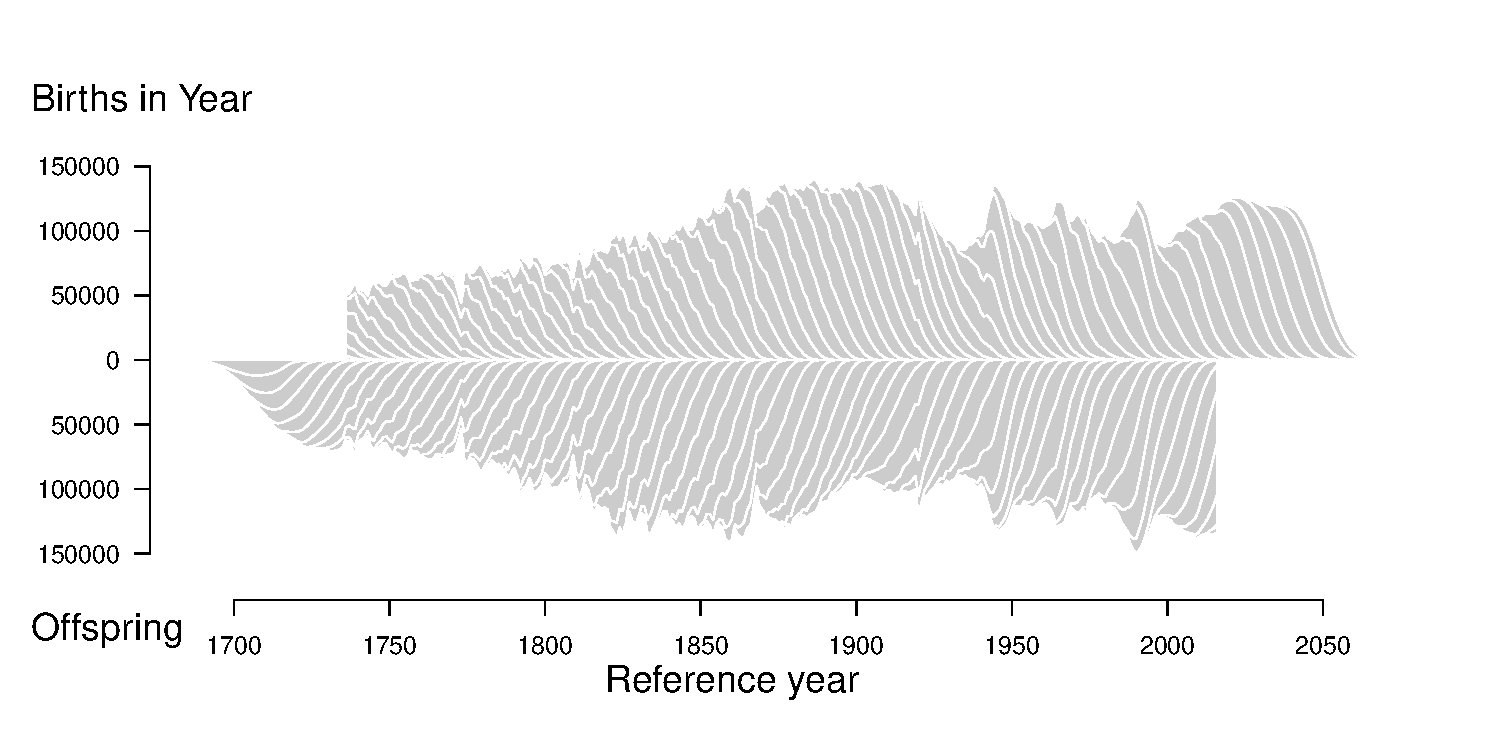
\includegraphics[width=\textwidth]{Figures/JoinBins.pdf}
        \caption{One time series of birth count distributions, under the period and cohort perspectives. The top series is composed of stacked polygons representing the quinquennial mother cohort birth distributions indexed to period. The bottom series is composed of stacked polygons representing quinquennial period birth distributions indexed to mothers' cohort. This is the underlying structure of fold-out Fig.~\ref{fig:foldout}.}
          \label{fig:joinbins}
\end{figure}